\chapter{Implementation}
\label{Implementation}
This chapter describes the implementation details of the system, shows the internal
architecture. As mentioned in the previous chapter, the program was created in Typescript, and they are using js-ipfs\footnote{\url{https://github.com/ipfs/js-ipfs}} implementation of IPFS node. This selection of tools enables code sharing between these two separated applications.

\section{Explorer-core implementation}
Explorer-core is the most complex module of a whole system with more than 5000 lines of code. The database is a main part of the explorer-core module. Database system consists of a query system, indexes and a database abstract layer. 

\subsection{Indexes}
For indexing there is currently implemented only B-tree, but different structures such as tries\footnote{\url{https://en.wikipedia.org/wiki/Trie}} can be implemented easily. They only need to implement index's interface (function such as \texttt{insert}, \texttt{delete}, \texttt{update}, \texttt{find}). We can create indexes on database entities with decorators\footnote{\url{https://www.typescriptlang.org/docs/handbook/decorators.html}}, which are part of ECMAScript 6 standard. Every database entity has to have \texttt{PrimaryKey} decorator on property that is used as a primary index. Index has three parameters:
\begin{itemize}
    \item \texttt{comparator} - is a function that accepts two arguments and returns number that is less than zero if first arguments is greater than second, zero if arguments are the same, more then zero if a second argument is greater than first. If a user has not set any custom comparator default one (\texttt{(a, b) =>
    a < b ? -1 : +(a > b)}) is used. This default comparator works on atomic keys such as string or numbers. 
    \item \texttt{keyGetter} - is another function that accepts a whole entity as arguments and returns key, that is used in an index. A default key getter is function that returns property of the entity (for example default key getter for property \texttt{height} is \texttt{(e) =>  e[''height'']}).
    \item \texttt{branching} - the branching factor is the number of children at each node, the outdegree. Default branching factor is 16.
\end{itemize}

\todo{Image of B-Tree}

\subsection{Query system}
Database system offers a complex query system. A query can consist of multiple conditions and the \texttt{Query Planner} is responsible for resolving them. It decides which indexes are used for query and choose a strategy. If there is no condition, a primary key is used for query execution. In the case of a single condition, \texttt{Query Planner} checks if there is an index on the condition's property. If yes, then this index is used to perform the query. Else condition is transformed to filter and a primary key is used to obtain results which are then filtered. For multiple conditions connected with logical operators \texttt{AND} or \texttt{OR}, \texttt{Query Planner} creates \texttt{OR-hashset} and \texttt{AND-hashset}. \texttt{AND-hashset} is initialized with the results of a condition which has the smallest number of results and uses \texttt{AND} operator. Then we check for each result hash for all other \texttt{AND} conditions if \texttt{AND-hashset} contains it. If no, a hash is deleted from \texttt{AND-hashset}. This creates intersection between all \texttt{AND} conditions. The \texttt{OR-hashset} is created empty. Then, we add a hash of every result of all \texttt{OR} conditions to it. This creates union between \texttt{OR} conditions. At the end, we perform union between \texttt{AND-hashset} and \texttt{OR-hashset}. This creates final hashset which is used later to obtain actual data with resolvers such as \texttt{all}, \texttt{first}, \texttt{paginate} etc. If one of the \texttt{AND} conditions has great selectivity (it has less than a hundred results), \texttt{Query Planner} can decide to don't use other indexes, but transform condition to filter and cycle over the results.

\subsection{Database}
The most important part of the explorer-core module is a Database system which connects query system with indexes. When we make a query, it translates to the database, and data are obtained from the indexes.

\subsubsection{Tables}
A database contains tables. A table contains indexes and table name and implements operations that modifies its state:
\begin{itemize}
    \item \texttt{insert} - creates history log for entity with first entity version. Then adds it to every table index.
    \item \texttt{update} - adds new version of the entity to its history log. Than update every index of the table.
    \item \texttt{delete} - removes entity from every table index. From now, entity can not be find in this table.
\end{itemize}

\subsubsection{Transactions}
A database can be executing only a single transaction at the time to prevent data inconsistency. For that reason, we implemented a transaction queue where transactions are stored before executing in the order in which they came. Executing more transactions in a row is significantly more effective than executing them one by one. If a transactions queue has only one transaction, it will wait 100ms for more transactions to come.  

\subsubsection{Synchronization}
There are two types of transactions. Those that changes the database state (\texttt{create}, \texttt{update}, \texttt{delete}) and those that don't (\texttt{read}). Every transaction that changes database state need to be synchronized with other peers. We created Database log for that. It is an append-only log with a discrete time. There can be only one valid database transaction in every point in time. There are several strategies to choose which transaction is globally accepted and which transactions need to rollbacks.

\begin{itemize}
    \item \textbf{Longer connected wins} - user that is connected to database 
\end{itemize}




\section{Feeder implementation}
A Feeder is a simple program (less than a hundred lines of code) written in Typescript (see Algorithm \ref{feederAlgo}). It strongly depends only explorer-core module. Currently, we support only Blockbook connector as a source of blockchain's data, but Feeder can be simply expanded to support more data source such as InsightAPI or direct connection to a blockchain as a full node. Each Feeder has configuration file (usually called \texttt{.env}) with Feeder's settings. Main Feeder settings are \texttt{URL} of the source for the blockchain's data and \texttt{DB\_NAME} which is a name of the database where Feeder inserts new blocks. A Feeder can be connected to only one blockchain (we can spawn one Feeder for every blockchain we want to index).



\begin{algorithm}[H]
    \SetAlgoLined
    load configuration\;
     \While{there is new block}{
         fetch block\;
         \For{transaction in block}{
            save transaction\;
            }
          save block\;
     }
    \caption{Feeder algorithm}
    \label{feederAlgo}
\end{algorithm}



\begin{itemize}
   
    \item \textbf{B+ Tree} - It is perhaps the most powerful index structure. With auto balanced B+ tree, we can efficiently search objects by given key and performs range selects. Example of this structure can be seen in Figure \ref{btreeindex}. By default, there is the limit of 32 items in one node (but can be changed from 4 to 256). 
    


    \begin{figure}[h]
        \centering
        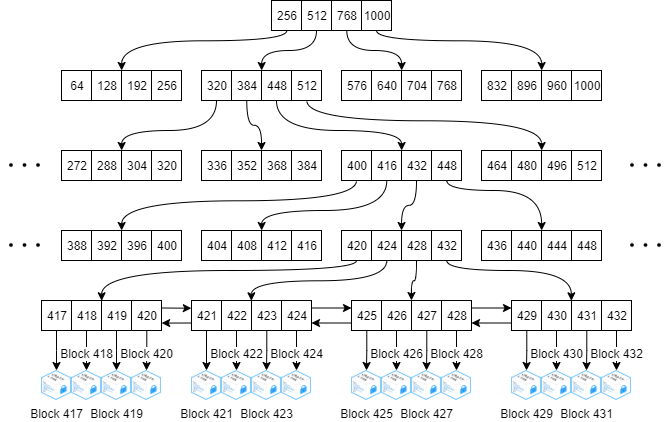
\includegraphics[width=13cm]{btreeindex.png}
        \caption{B+ tree index structure}
        \label{btreeindex}
        \todo{Change image of B-tree without cyclic references}
    \end{figure}

\end{itemize}
Implementing these indexes in IPFS was surprisingly simple thanks to IPLD objects and links. When Feeder stores data into IPFS, it may also perform an index update that will change content address of the index. To prevent this, we use IPNS for creating and updating mutable links to indexes.



\section{Explorer implementation}
We can split Explorer to several modules. The central part is ExplorerCore which communicates with IPFS and provides an interface to explore blockchain and to perform queries. There can be ExplorerGUI or ExplorerAPI on the top of the ExplorerCore. These modules are providing communication with user or other systems. This architecture is shown in Figure \ref{ExplorerArchitecture}.

\begin{figure}[h]
    \centering
    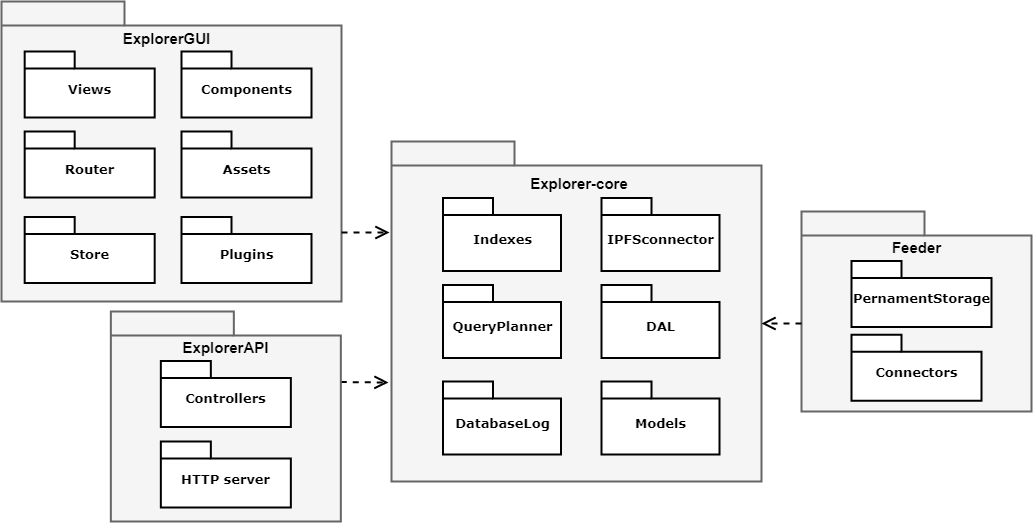
\includegraphics[width=13cm]{ExplorerArchitecture.png}
    \caption{Explorer architecture}
    \label{ExplorerArchitecture}
\end{figure}

\subsection{ExplorerCore}
ExplorerCore is main module of the Explorer. It is responsible for obtaining and resolving data from IPFS and performing queries. It has simple interface:
\begin{itemize}
    \item \texttt{getObject(CID[, path])} - gets object from IPFS with optional path,
    \item \texttt{getTx(txHash)} - gets transaction by its hash,
    \item \texttt{getBlock(blockHash)} - gets block by its hash,
    \item \texttt{getBlock(blockHeight)} - gets block by its height,
    \item \texttt{getAddress(addressHash)} - gets address by its hash.
\end{itemize}
All ExplorerCore methods except \texttt{getObject} are returning \texttt{QueryObject}.

\subsubsection{Query system}
Explorer supports a simple query system. Every queriable object (address, transaction, block) has methods:
\begin{itemize}
    \item \texttt{where(propertyName)} - create a condition on the property. There can be multiple conditions in one query. A condition hash to be followed by one of the functions: 
    \begin{itemize}
        \item \texttt{gt(value)} - property is greater or equal than \texttt{value}. The query finds in an index first object that has property (set by \texttt{propertyName} in condition) equal or greater than \texttt{value}, and traverse index to the right (to bigger objects).
        \item \texttt{lt(value)} - property is less or equal than \texttt{value}. Similar as in the \texttt{gt} function, the query finds the closest object that has property equal or less than \texttt{value}. Then, the query traverses index to the smaller objects with smaller index value (to the left).
        \item \texttt{between(min, max)} - property is greater or equal than \texttt{min} and less or equal than \texttt{max}. 
    \end{itemize}
    \item \texttt{offset(offsetValue)} - query will skip \texttt{offsetValue} number of results,
    \item \texttt{limit(limitValue)} - set maximum number of results. After query has \texttt{limitValue} count of matched objects it will stop browsing the index,
    \item \texttt{all()} - return all objects that matched query,
    \item \texttt{first()} - return the first object that matched a query,
    \item \texttt{and(childQuery)} - logical and between two queries. Parent query resolves \texttt{childQuery} (call \texttt{all()} function) and makes a hashtable from its results. Later, when parent query being resolved, query checks if the result exists in the hashtable for every result.
    \item \texttt{or(childQuery)} - logical or between two queries. \texttt{childQuery} will be resolved by parent query, and its results stores in hashtable. When the parent query is resolved, its results will be added to the hashtable. This will remove duplicates in the final results.
    \item \texttt{[Symbol.iterator]()} - iterator that is used in cycle \texttt{for (result of query)}.

\end{itemize}

The data obtaining will happen only when we access the data inside the Query object (for example, in for-loop) or by calling \texttt{all()} or \texttt{first()} method. Index is used only for the first condition in a query, that is on the property, that has created index. Other conditions are performed client-side.

\subsection{ExplorerGUI}
ExplorerGUI is a single page application with simple user interface that runs in browser implemented with Vue.js\footnote{\url{https://vuejs.org/}}. Browser's implementation of IndexedDB is used as a storage for IPFS as can be seen in Figure \ref{browserIPFS}. Communication with other peers is provided though WebRTC\footnote{\url{https://webrtc.org/}} or WebSockets. Every tab opened in the browser is the same IPFS node. Opening a new tab in Incognito mode or different browser will spawn different IPFS node.

\begin{figure}[h]
    \centering
    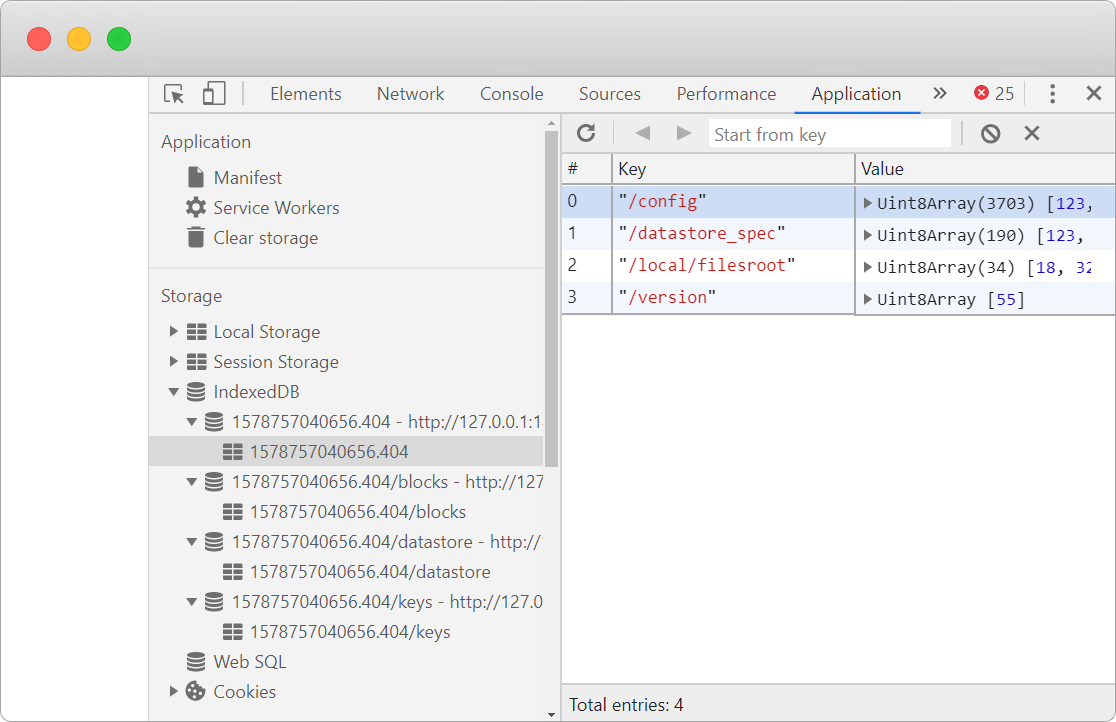
\includegraphics[width=12cm]{ipfsBrowser.PNG}
    \caption{IPFS storage in browser}
    \label{browserIPFS}
\end{figure}


\subsection{ExplorerAPI}
Node.js\footnote{\url{https://nodejs.org/}} implementation of IPFS uses filesystem to store data (see Figure \ref{nodeIPFS}). On the top of ExplorerCore, there is a simple web framework Express\footnote{\url{http://expressjs.com/}}, where are routes (endpoints) defined. Currently available routes are described in Section \ref{explorerAPIroutes}. Every route supports query parameters \texttt{filter} (used for filtering results) and \texttt{limit} (which reduces number of results). Pagination can be made by setting \texttt{filter} to be greater/smaller (depending on ordering) as key of the last displayed object and \texttt{limit} to page size. For example, if a user is looking at page of transactions ordered by time (ordered from the newest transactions to the oldest), the next page of transactions are first \(N\) transactions that happened before last displayed transaction (where \(N\) is page size).

Rest API supports optional path param \texttt{path} that is useful for traversing objects in IPFS. If we want to get fifth transaction of the block with height 1000 one of the way is request URL \texttt{/block/998/next\_block/next\_block/txs/5} (get block with height 998, get next block two times, get transaction, a get fifth item from array of transactions). This approach allows the user to explore IPFS storage as graph very quickly by objects links.

\begin{figure}[h]
    \centering
    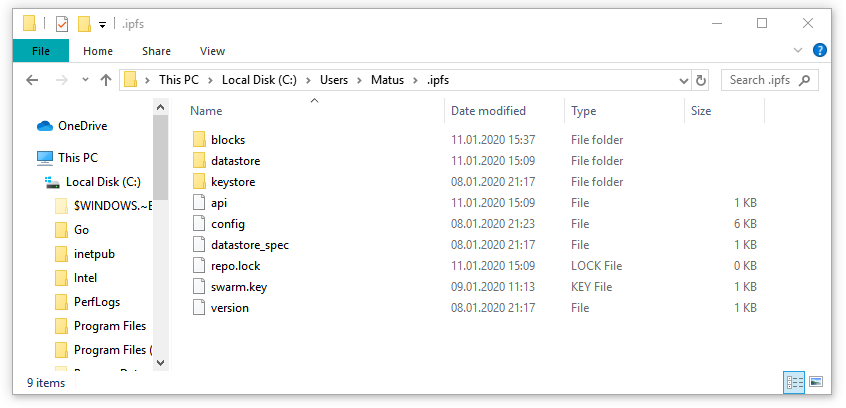
\includegraphics[width=12cm]{ipfsNode.PNG}
    \caption{IPFS storage in node.js}
    \label{nodeIPFS}
\end{figure}
